\section{Questionnaire \& Practical Examples}

\begin{questionbox}[Question 1]
\textit{What are the advantages and disadvantages of using the unified system call interface for manipulating different system components (read/write/free for files, memory, and I/O devices)? Consider how this abstraction influences OS design, performance trade-offs, error handling complexity, and the balance between portability and efficiency.}
\end{questionbox}

\textbf{Answer:}\\
The Unix philosophy of \textit{``everything is a file''} abstracts all I/O resources (disks, sockets, pipes, terminals, memory-mapped devices) into a uniform \texttt{file descriptor} handle. Every resource is manipulated via a small set of system calls: \texttt{open()}, \texttt{read()}, \texttt{write()}, \texttt{close()}.

\textbf{Internal Architecture (VFS Layer):}\\
The kernel implements this via the \textbf{Virtual File System (VFS)}, a software indirection layer that maps each syscall to a driver-specific handler through a table of function pointers (\texttt{struct file\_operations}). When a user calls \texttt{write(fd, buf, n)}, the VFS dispatches to the correct handler---whether that is a hard disk driver, a network socket, or a GPU device---without the user knowing which:
\begin{lstlisting}[language=C]
struct file_operations {
    ssize_t (*read)(struct file *, char __user *, size_t, loff_t *);
    ssize_t (*write)(struct file *, const char __user *, size_t, loff_t *);
    int     (*open)(struct inode *, struct file *);
    int     (*release)(struct inode *, struct file *);
};
\end{lstlisting}

\begin{itemize}
    \item \textbf{Advantages:}
    \begin{itemize}
        \item \textit{Portability \& Composability:} A utility like \texttt{cat} that reads \texttt{stdin} works identically whether stdin is a file, a pipe, or a network socket. No code changes are needed.
        \item \textit{Unified Security Model:} POSIX permission bits (\texttt{rwxr-xr-x}) and \texttt{DAC/MAC} policies apply uniformly to all resources through a single mechanism.
        \item \textit{Simplified OS Design:} The kernel only needs one generic buffer-cache subsystem, one locking strategy, and one error-propagation pathway to cover all device types.
        \item \textit{In our OS:} The instruction dispatcher in \texttt{cpu.c} handles \texttt{READ}/\texttt{WRITE}/\texttt{FREE} opcodes directly, while the \texttt{SYSCALL} opcode transitions to kernel mode and routes through \texttt{libsyscall()} and \texttt{\_syscall()} (syscall table in \texttt{syscall.c}). The unification point is therefore the syscall layer, not a per-opcode table in \texttt{cpu.c}.
    \end{itemize}
    \item \textbf{Disadvantages:}
    \begin{itemize}
        \item \textit{Performance Overhead:} Every access passes through VFS indirection layers. A direct memory-mapped I/O (\texttt{mmap}) bypasses this cost entirely, which is why high-performance databases (e.g., PostgreSQL) prefer \texttt{mmap} over \texttt{read()}.
        \item \textit{Imperfect Abstractions:} Network devices require connection state, asynchronous events, and specialized options that cannot fit cleanly into \texttt{read}/\texttt{write}. This forces the use of \texttt{ioctl()} --- an escape hatch that is opaque, non-portable, and notoriously hard to use correctly.
        \item \textit{Error Handling Complexity:} A single \texttt{write()} return value of \texttt{-1} must cover disk-full, network-reset, permission-denied, and hardware-fault conditions. Distinguishing these via \texttt{errno} alone is brittle.
    \end{itemize}
\end{itemize}

\begin{figure}[H]
    \centering
    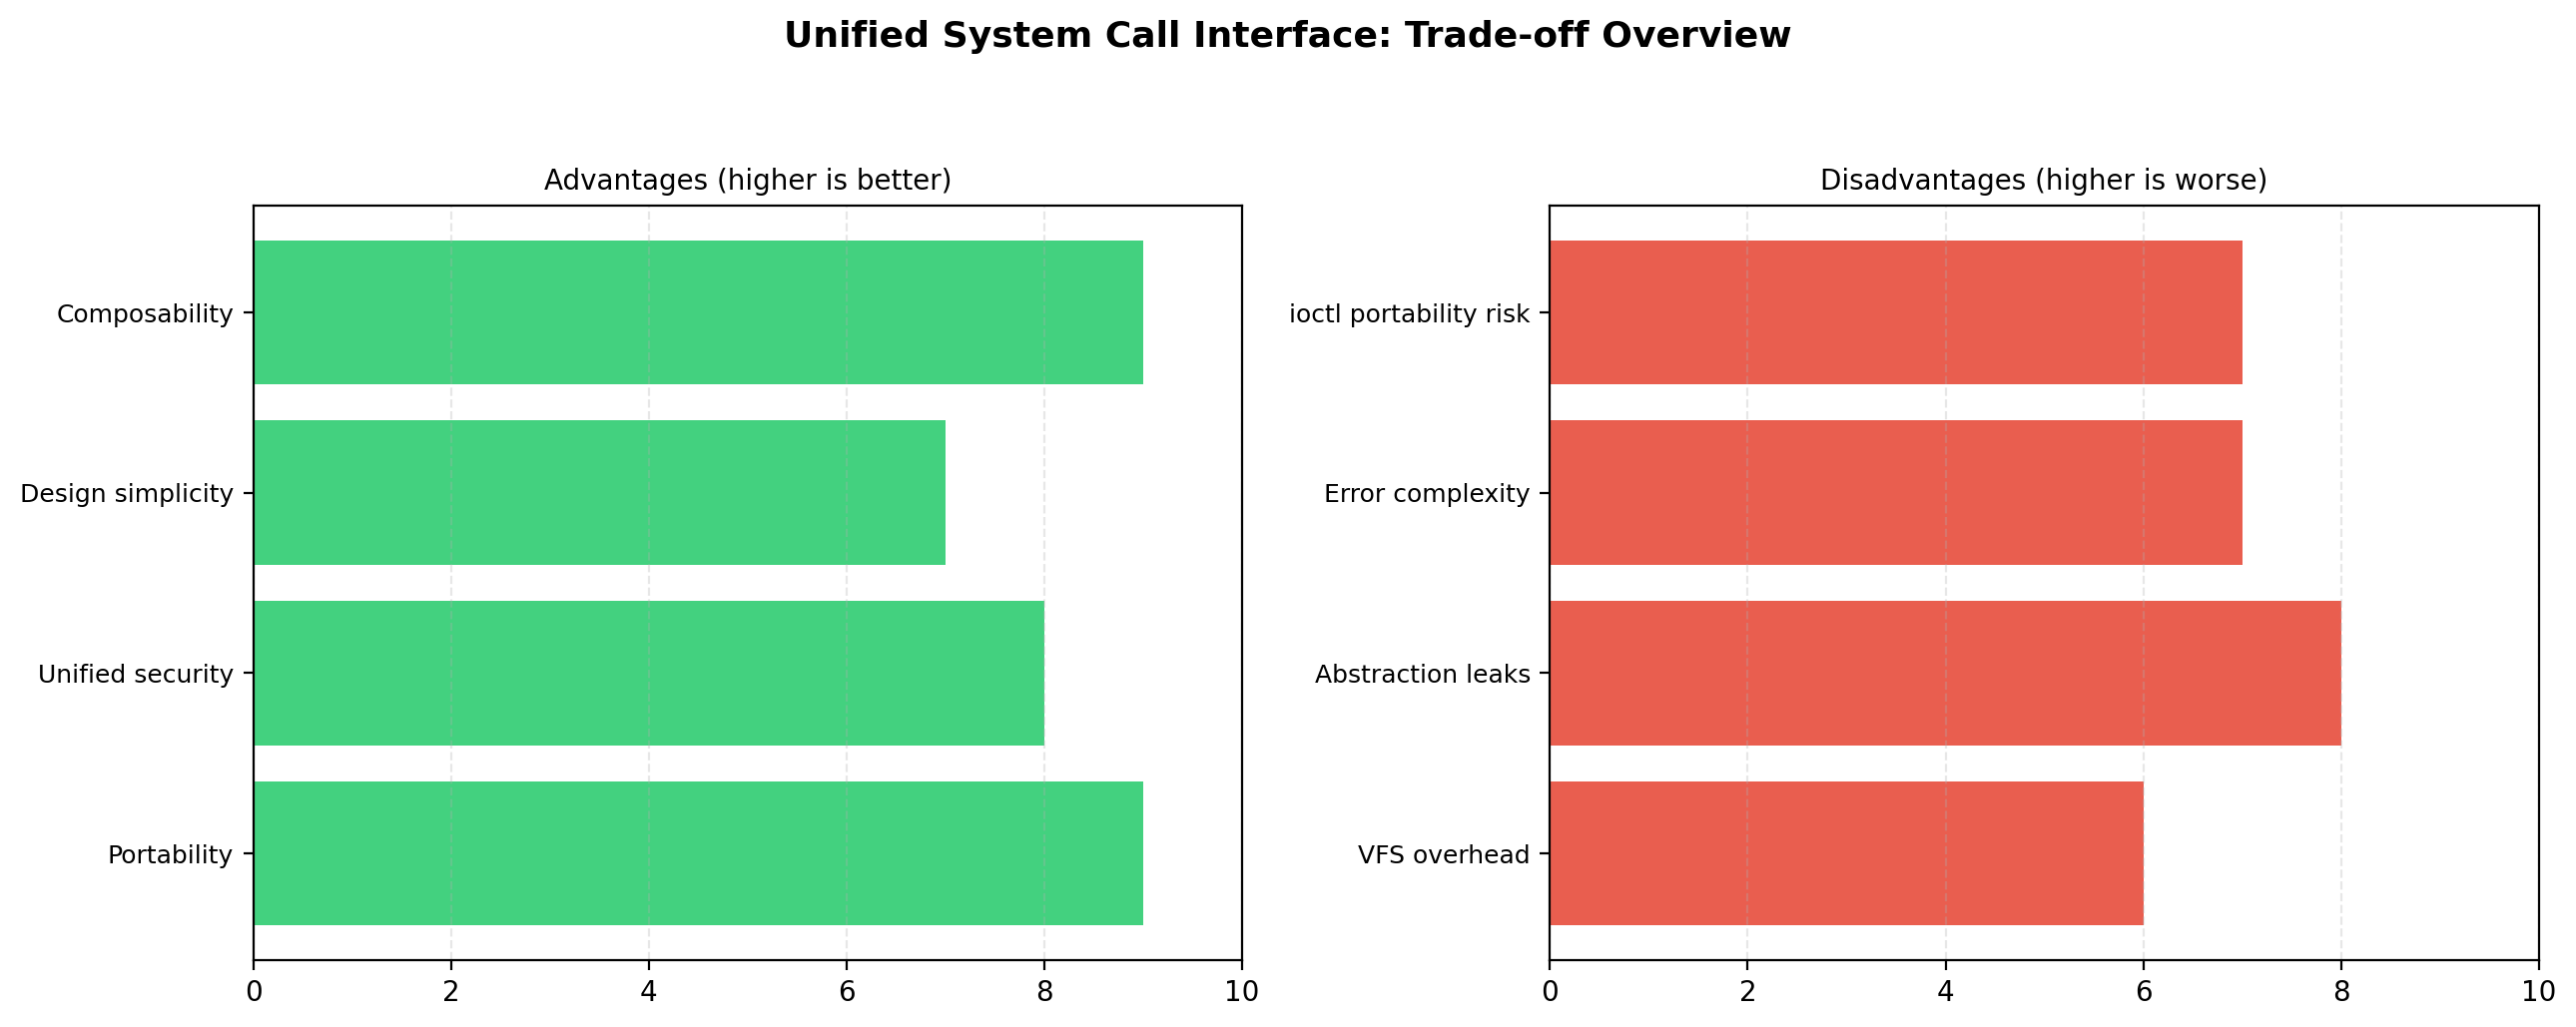
\includegraphics[width=0.9\linewidth]{Images/q1_viz.png}
    \caption{Question 1 summary map: major benefits and major trade-offs of the unified syscall interface.}
\end{figure}

\begin{questionbox}[Question 2]
\textit{When a system call executes too long, how does the Operating System detect and handle the case?}
\end{questionbox}

\textbf{Answer:}\\
When a user process issues a system call (\texttt{SYSCALL} instruction), the CPU switches to kernel mode, saves register state, and executes kernel code. While executing kernel code, if the system call blocks forever (e.g., waiting on a broken I/O device, or spinning in an infinite loop in a buggy driver), it can hang the entire CPU core, starving all other processes.

\textbf{Hardware-Driven Detection: The APIC Timer}\\
Modern CPUs include a local \textbf{APIC (Advanced Programmable Interrupt Controller)} timer. The OS programs this timer to fire a periodic interrupt---typically every 1ms to 10ms (the ``tick''). This interrupt fires regardless of whether the CPU is in user mode or kernel mode. The tick handler is the scheduler's heartbeat:
\begin{enumerate}
    \item \textbf{Timer Arms:} Before dispatching a process, the OS records \texttt{dispatch\_time} and sets the APIC for the next tick.
    \item \textbf{Tick Fires:} At every tick, the CPU saves context (all registers, instruction pointer, stack pointer) and jumps to the interrupt service routine (ISR).
    \item \textbf{Scheduler Evaluates:} The ISR checks: has the current process exceeded its time quantum? If yes, \textbf{preempt} it: save its state, place it back on the ready queue, and schedule the next runnable process.
    \item \textbf{Deadlock / Soft Lockup Detection (Linux reference):} Linux may use watchdog-based lockup detection to report stuck CPUs. Our simulator does not implement a dedicated watchdog thread; instead, progress is controlled by deterministic time-slice preemption in the scheduler loop.
\end{enumerate}

\begin{figure}[H]
    \centering
    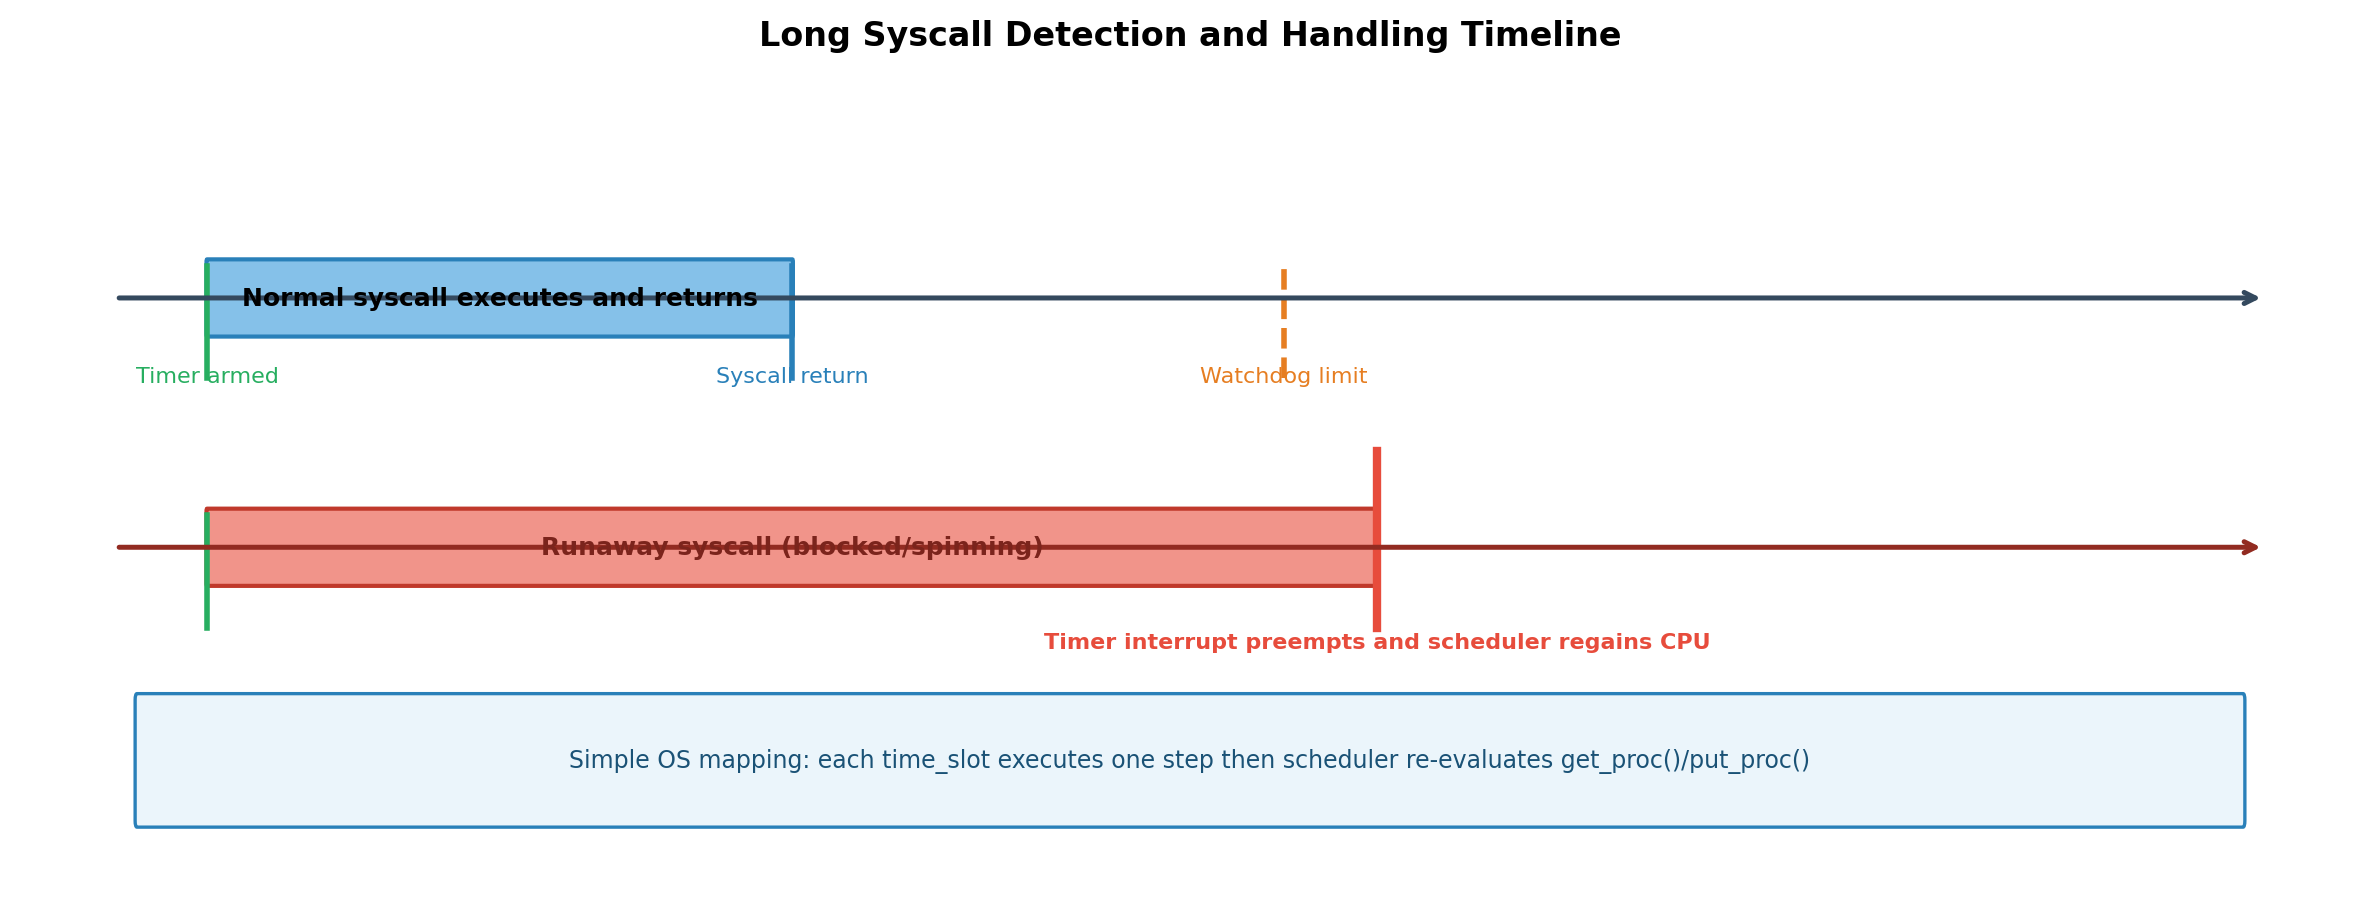
\includegraphics[width=0.95\linewidth]{Images/q2_watchdog.png}
    \caption{Timeline showing a normal syscall completing before the watchdog limit vs. a runaway syscall intercepted by the hardware timer interrupt.}
\end{figure}

\textbf{Relevance to our Simple OS:}\\
In \texttt{os.c}, each CPU thread runs a scheduling loop. The \texttt{time\_slot} counter plays the role of the hardware timer tick. After each time slot, the scheduler evaluates whether to preempt the running process:
\begin{lstlisting}[language=C]
while (1) {
    time_slot++;
    proc = get_proc_from_run_list(cpu_id);
    if (proc) run(proc);  // one instruction
    // Implicit preemption: move back to MLQ
    add_proc_to_ready_queue(proc);
}
\end{lstlisting}
Because each CPU executes only \textit{one instruction per slot}, no single system call can monopolize the CPU for more than one tick---this is the Simple OS's equivalent of APIC-driven preemption.

\begin{questionbox}[Question 3]
\textit{Considering the impactness of MLQ detailed policies, what is the benefit of each policy?}
\end{questionbox}

\textbf{Answer:}\\
The Multi-Level Queue (MLQ) scheduler in \texttt{sched.c} combines three distinct policies to balance responsiveness, fairness, and throughput simultaneously:

\textbf{Policy 1: Strict Priority-Ordered Queues}\\
The scheduler iterates from priority level 0 up to \texttt{MAX\_PRIO - 1} and always dispatches from the highest non-empty queue (\texttt{get\_mlq\_proc()}). This ensures that real-time and interactive processes (low priority number) are never delayed by compute-bound background jobs.

\textbf{Policy 2: Time-Sliced Round Robin Within Each Queue}\\
Processes at the same priority level are served in FIFO/Round Robin order. Each dequeued process runs for its fully allocated time slice (e.g., 2 ticks), then is re-enqueued (via put\_mlq\_proc()) . This prevents any single process from monopolizing its priority level.

\textbf{Policy 3: Slot Budget Exhaustion \& Reset (Starvation Prevention)}\\
Each priority queue is assigned a budget of \texttt{MAX\_PRIO - prio} slots (higher priority $\rightarrow$ more budget). Once a queue's budget hits zero, it is skipped until \textit{all} queues are exhausted, at which point all budgets reset. This is the key anti-starvation mechanism.

\textbf{Empirical Proof from our actual output:}\\
The following trace from \texttt{sched\_0.actual.output} shows three distinct policy interactions. PID 1 and 2 share the same priority (PRIO 4). PID 3 and 4 have higher priority (PRIO 0):
\begin{verbatim}
Time slot   1:  CPU 0: Dispatched process  1  (PRIO 4)
Time slot   3:  CPU 0: Put process  1 to run queue
                CPU 0: Dispatched process  2  <- Round Robin within PRIO 4
Time slot   4:                             [PID 3 loaded, PRIO 0 -- higher priority!]
Time slot   5:  CPU 0: Put process  2 to run queue
                CPU 0: Dispatched process  3  <- PRIO 0 preempts PRIO 4
Time slot   7:  CPU 0: Put process  3 to run queue
                CPU 0: Dispatched process  4  <- PRIO 0, Round Robin with PID 3
\end{verbatim}
\textbf{Key insight:} The P1$\to$P2 switch at Time Slot 3 is \textbf{intra-queue Round Robin}: both processes share PRIO 4, so after PID 1's time slice expires, PID 2 (next in the same queue) runs. The P2$\to$P3 switch at Time Slot 5 is \textbf{higher-priority preemption}: PID 3 was loaded at Time Slot 4 into the PRIO 0 queue (budget = 140), which outranks PRIO 4 (budget = 136) in \texttt{get\_mlq\_proc()}'s linear scan.

\begin{figure}[H]
    \centering
    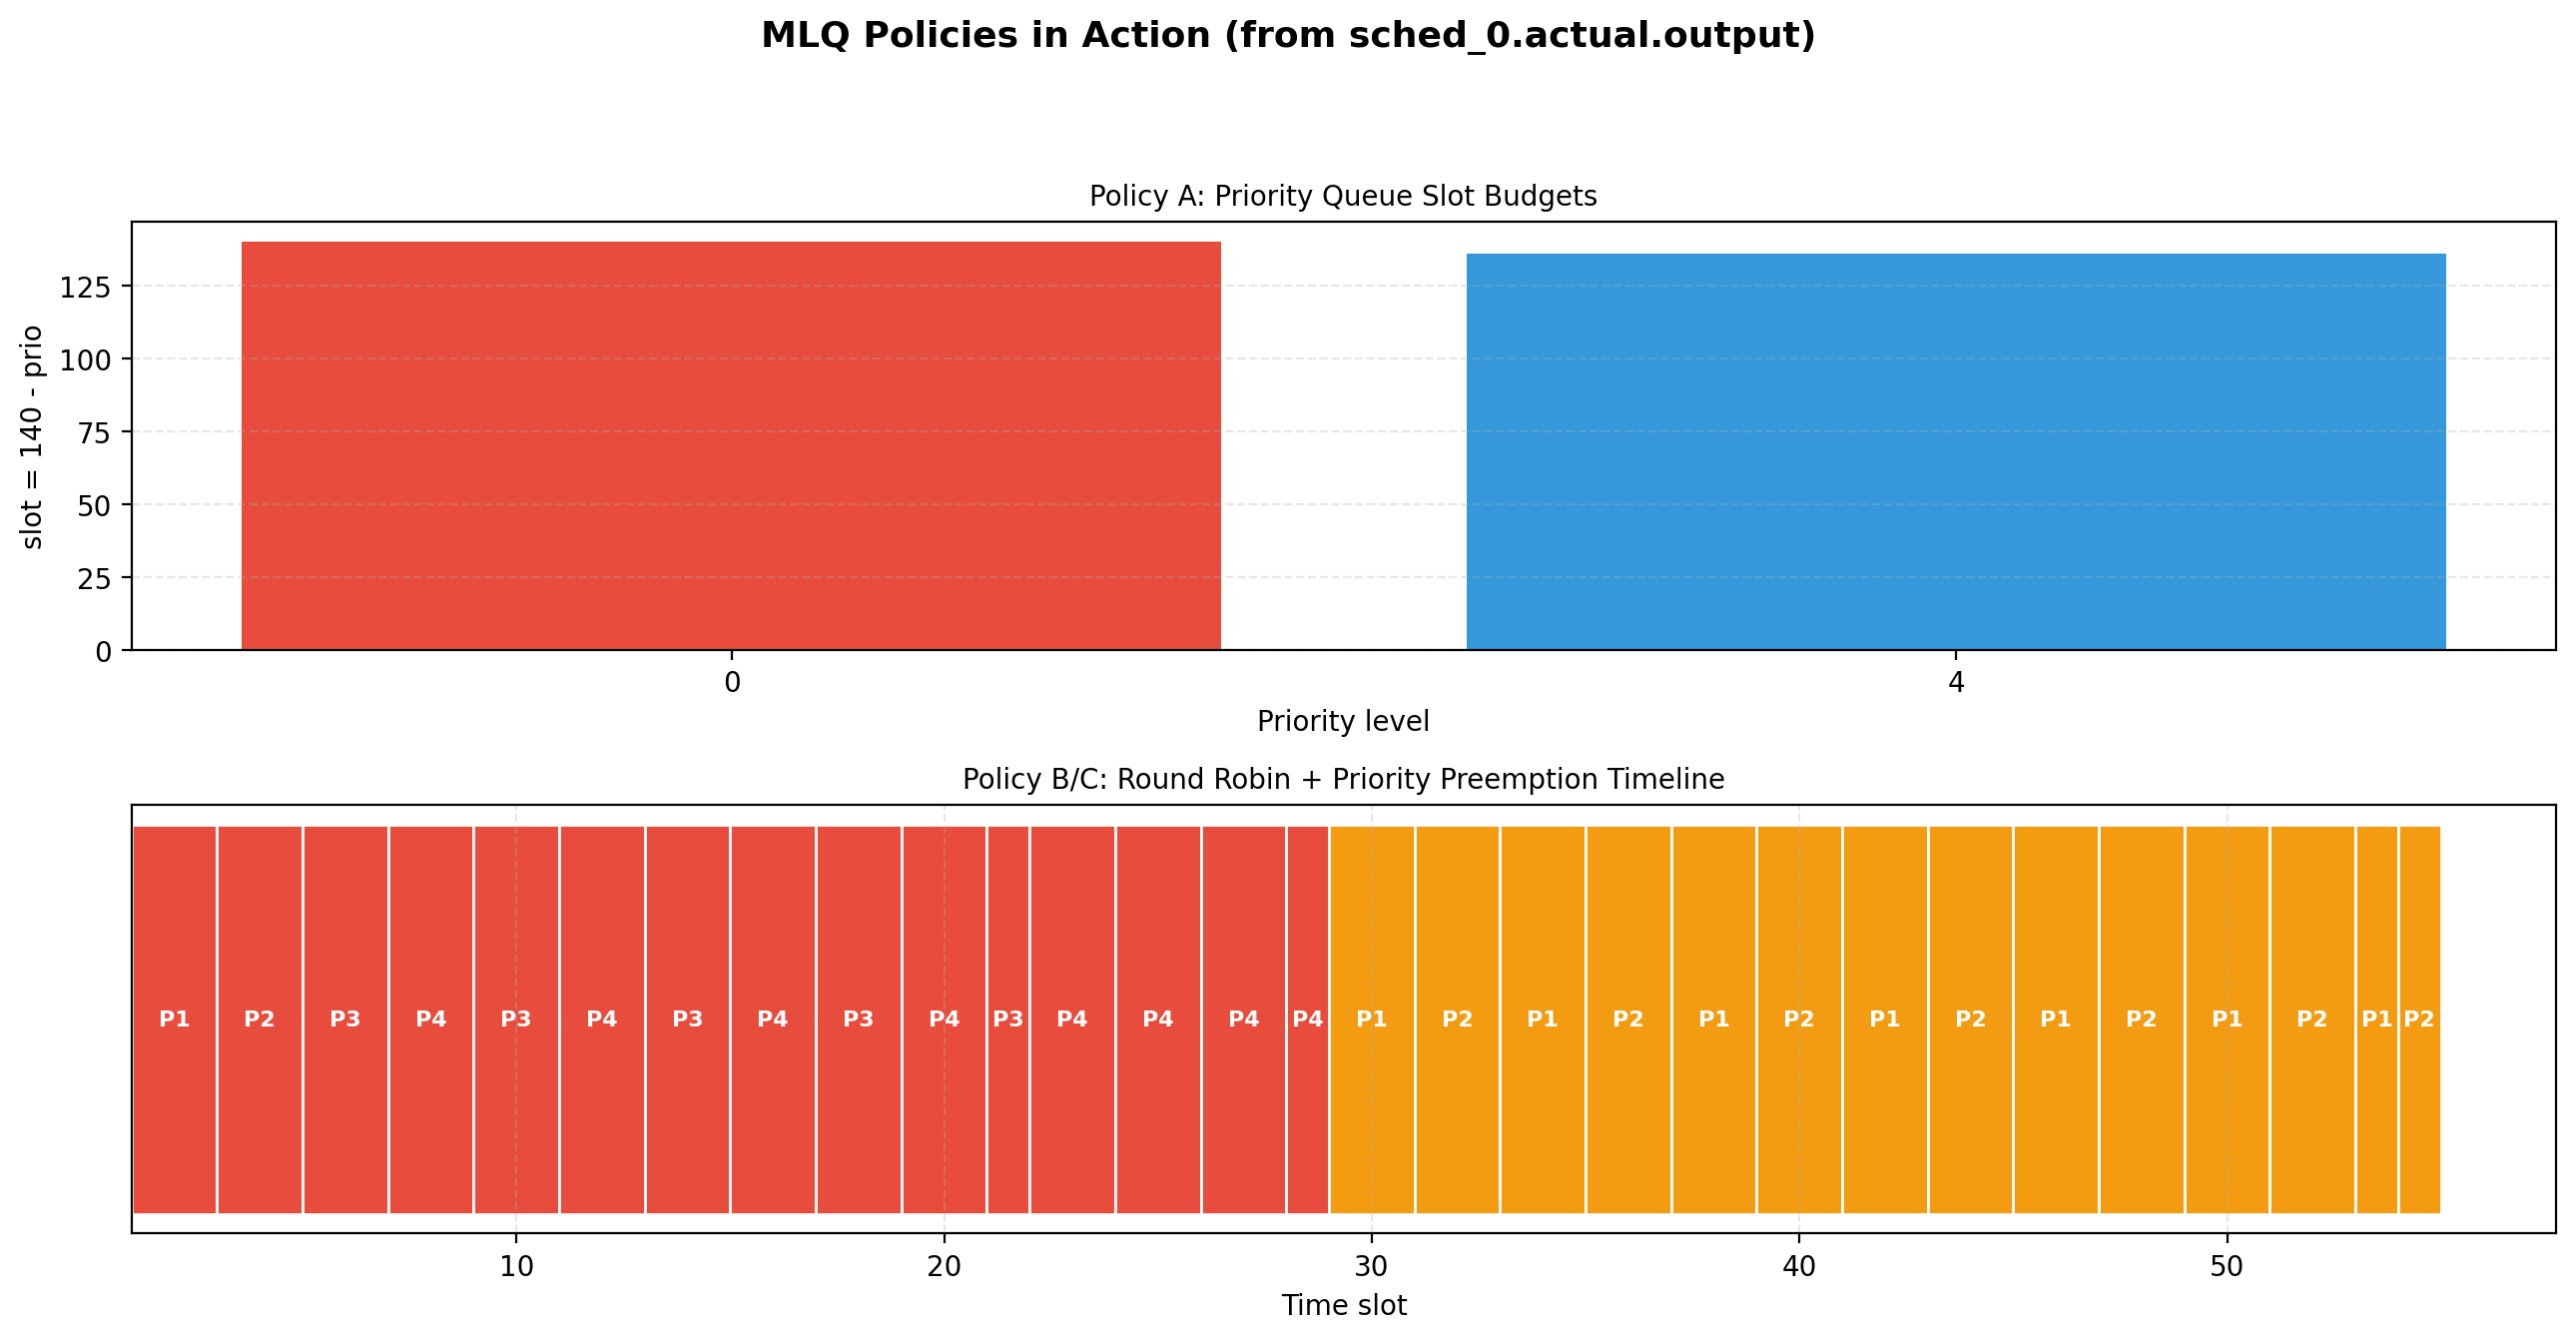
\includegraphics[width=0.9\linewidth]{Images/q3_viz.png}
    \caption{Question 3 evidence view: priority budget structure and actual scheduler timeline showing Round Robin and priority preemption.}
\end{figure}

\begin{questionbox}[Question 4]
\textit{What is the primary motivation for combining segmentation with paging in memory management? How does this hybrid approach address limitations inherent in using either technique alone?}
\end{questionbox}

\textbf{Answer:}\\
\textbf{The Core Problem:}\\
Pure segmentation gives programmers logical structure but causes \textit{external fragmentation}. Pure paging eliminates fragmentation but loses \textit{logical meaning and security boundaries}. The hybrid approach inherits the strengths of both.

\begin{itemize}
    \item \textbf{Segmentation Alone -- The Fragmentation Problem:}\\
    Each process is divided into variable-size segments (Code, Data, Heap, Stack). As processes start and stop, RAM becomes riddled with unusable holes. Example: 3 segments of 100KB each leave 50KB gaps between them. A new 200KB process cannot fit despite 150KB of total free space being available.

    \item \textbf{Paging Alone -- The Security Problem:}\\
    Paging divides everything into fixed 4KB frames. A single page might span both executable code and writable data. Without segment-level protections, a stack overflow can overwrite the code segment---the classic \textbf{Buffer Overflow attack vector}.

    \item \textbf{The Hybrid Solution (Intel x86):}\\
    The CPU first translates a logical address through the \textbf{GDT/LDT} (Segment Descriptor Tables) to produce a \textit{linear} address with access rights. Then the MMU translates that linear address through the multi-level page tables (via CR3) to produce the final \textit{physical} address. The two-step process:
    \[
    \underbrace{\text{Seg Base} + \text{Offset}}_{\text{Segmentation (GDT)}} \rightarrow \text{Linear Addr} \xrightarrow{\text{Page Tables (CR3)}} \text{Physical Addr}
    \]
\end{itemize}

\textbf{In our Simple OS:}\\
Each process owns a \texttt{struct mm\_struct} containing multiple \texttt{vm\_area\_struct} segments (VMA 0 = heap). Each VMA tracks its own \texttt{vm\_freerg\_list} for fast region search. When the heap must grow, \texttt{inc\_vma\_limit()} expands the VMA boundary and calls \texttt{vm\_map\_ram()} to back the new pages with physical frames---precisely the hybrid model.

\begin{figure}[H]
    \centering
    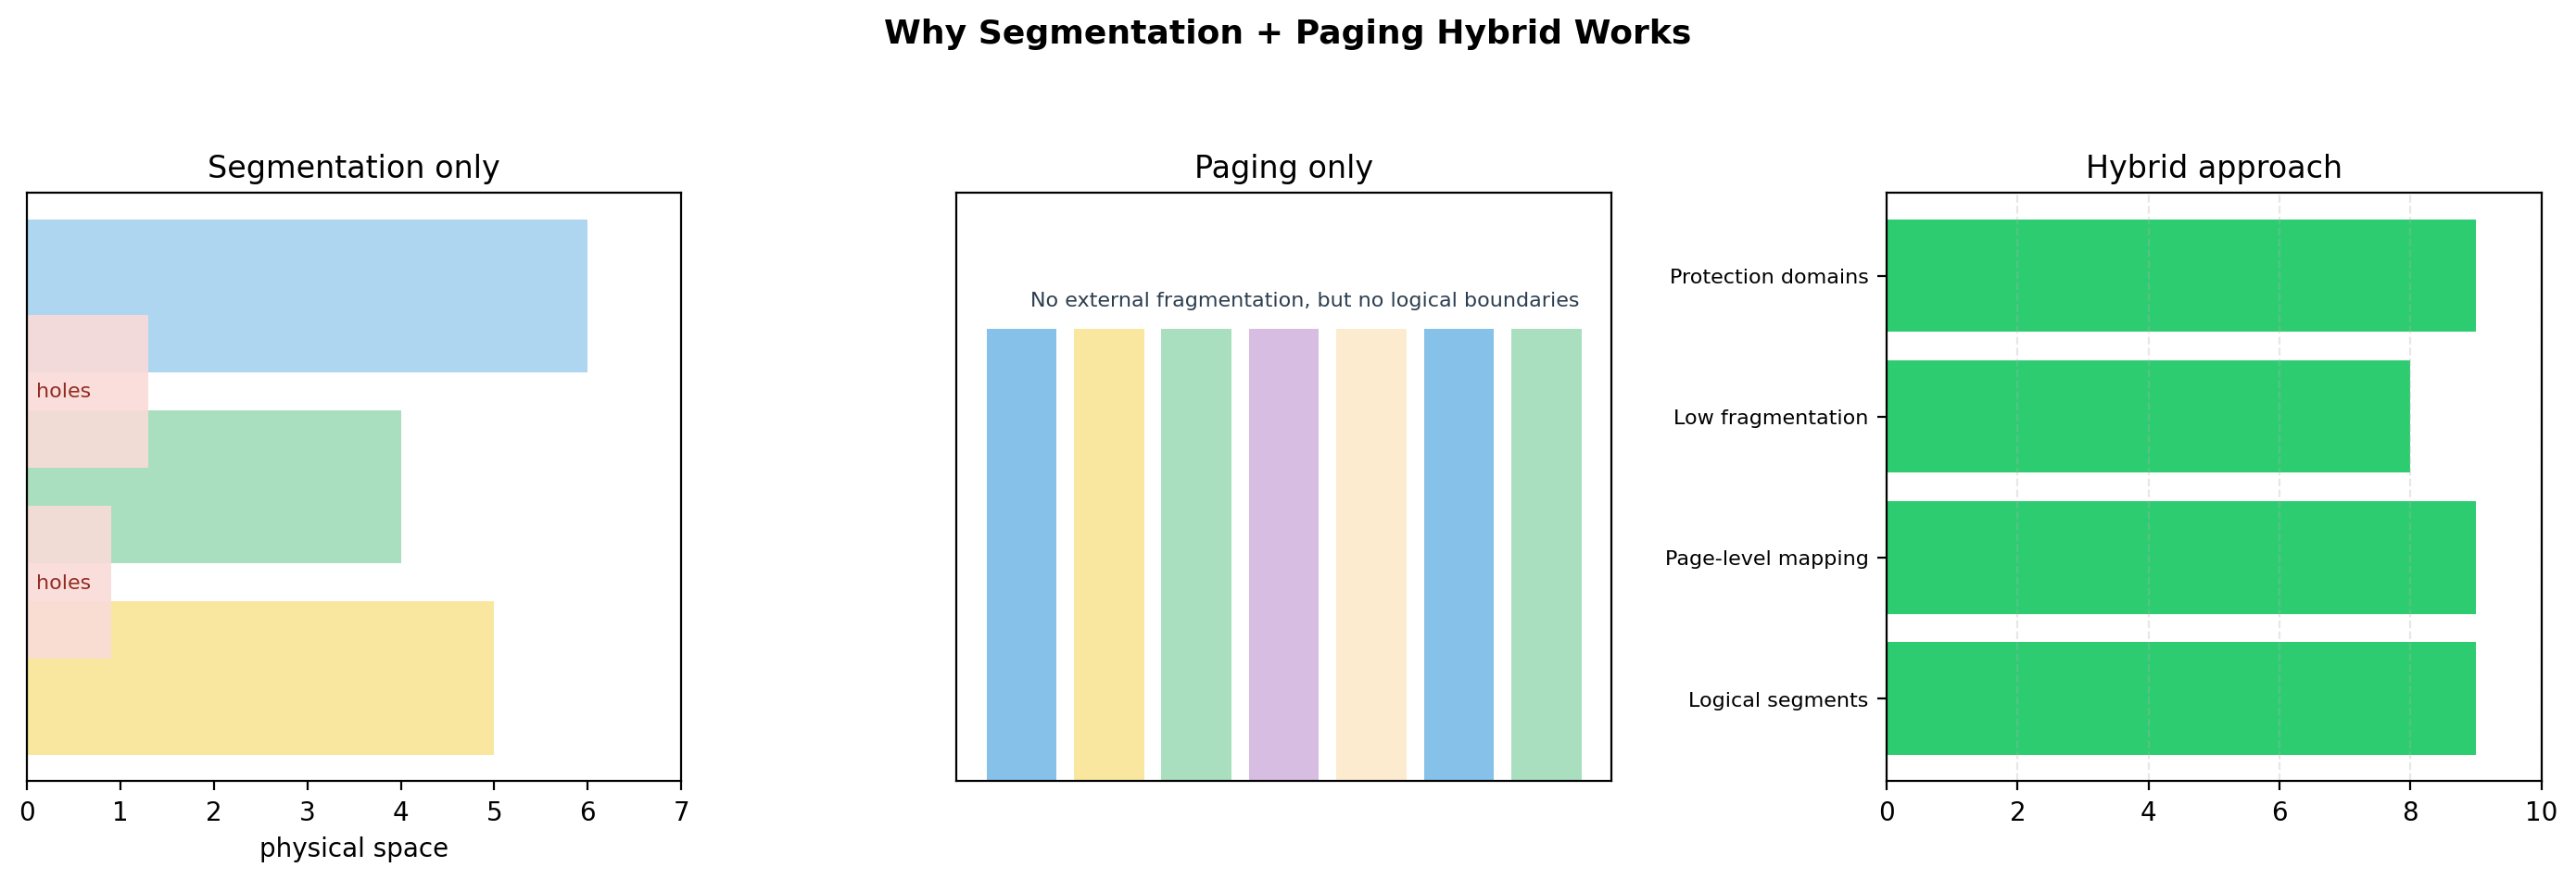
\includegraphics[width=0.9\linewidth]{Images/q4_segmentation_paging.png}
    \caption{Segmentation provides logical Code/Data boundaries; Paging maps those segments to non-contiguous 4KB physical frames, eliminating external fragmentation.}
\end{figure}

\begin{questionbox}[Question 5]
\textit{What are the benefits of extending hierarchical paging to N level?}
\end{questionbox}

\textbf{Answer:}\\
\noindent\textbf{The Scalability Problem:} \\
A 64-bit virtual address space contains $2^{64}$ bytes (16 Exabytes) of addressable memory. With 4KB pages, the number of virtual pages is $2^{52}$. A flat (single-level) page table storing 8 bytes per entry would require $2^{52} \times 8 = 32$ Petabytes per process, which is impractical to allocate.

\vspace{0.8em}
\noindent\textbf{N-Level Paging Solution:} \\
Hierarchical paging addresses this scalability issue by organizing page tables into multiple levels (PGD $\to$ P4D $\to$ PUD $\to$ PMD $\to$ PT). In a production operating system, only the portions of the hierarchy corresponding to active virtual address regions need to be populated, significantly reducing the amount of page-table data that must be actively maintained.

\vspace{0.8em}
\noindent\textbf{Design Decision in Our Simulator:} \\
While modern operating systems such as Linux implement true sparse hierarchical page tables, our Simple OS simulator adopts a different design trade-off. In \texttt{mm64.c}, the backing structures for all five paging levels are allocated as fixed-size flat arrays using \texttt{calloc()} during \texttt{init\_mm()}.

\begin{itemize}
    \item \textbf{Trade-off (Simplicity and Direct Indexing):} We sacrifice the memory efficiency of a fully sparse hierarchy in favor of a simpler implementation and direct array-based indexing. This approach avoids the complexity of dynamically allocating and managing lower-level page-table structures while preserving the logical organization of hierarchical paging.
    
    \item \textbf{Hierarchical Emulation:} Although the storage is preallocated, the simulator still follows the logical behavior of a 5-level paging system. Paging entries are marked as present only when a virtual page is mapped, and address translation proceeds through PGD, P4D, PUD, PMD, and PT indices exactly as in a hierarchical design. This demonstrates the correctness of the multi-level translation mechanism while keeping the implementation lightweight and suitable for educational simulation.
\end{itemize}

\begin{figure}[H]
    \centering
    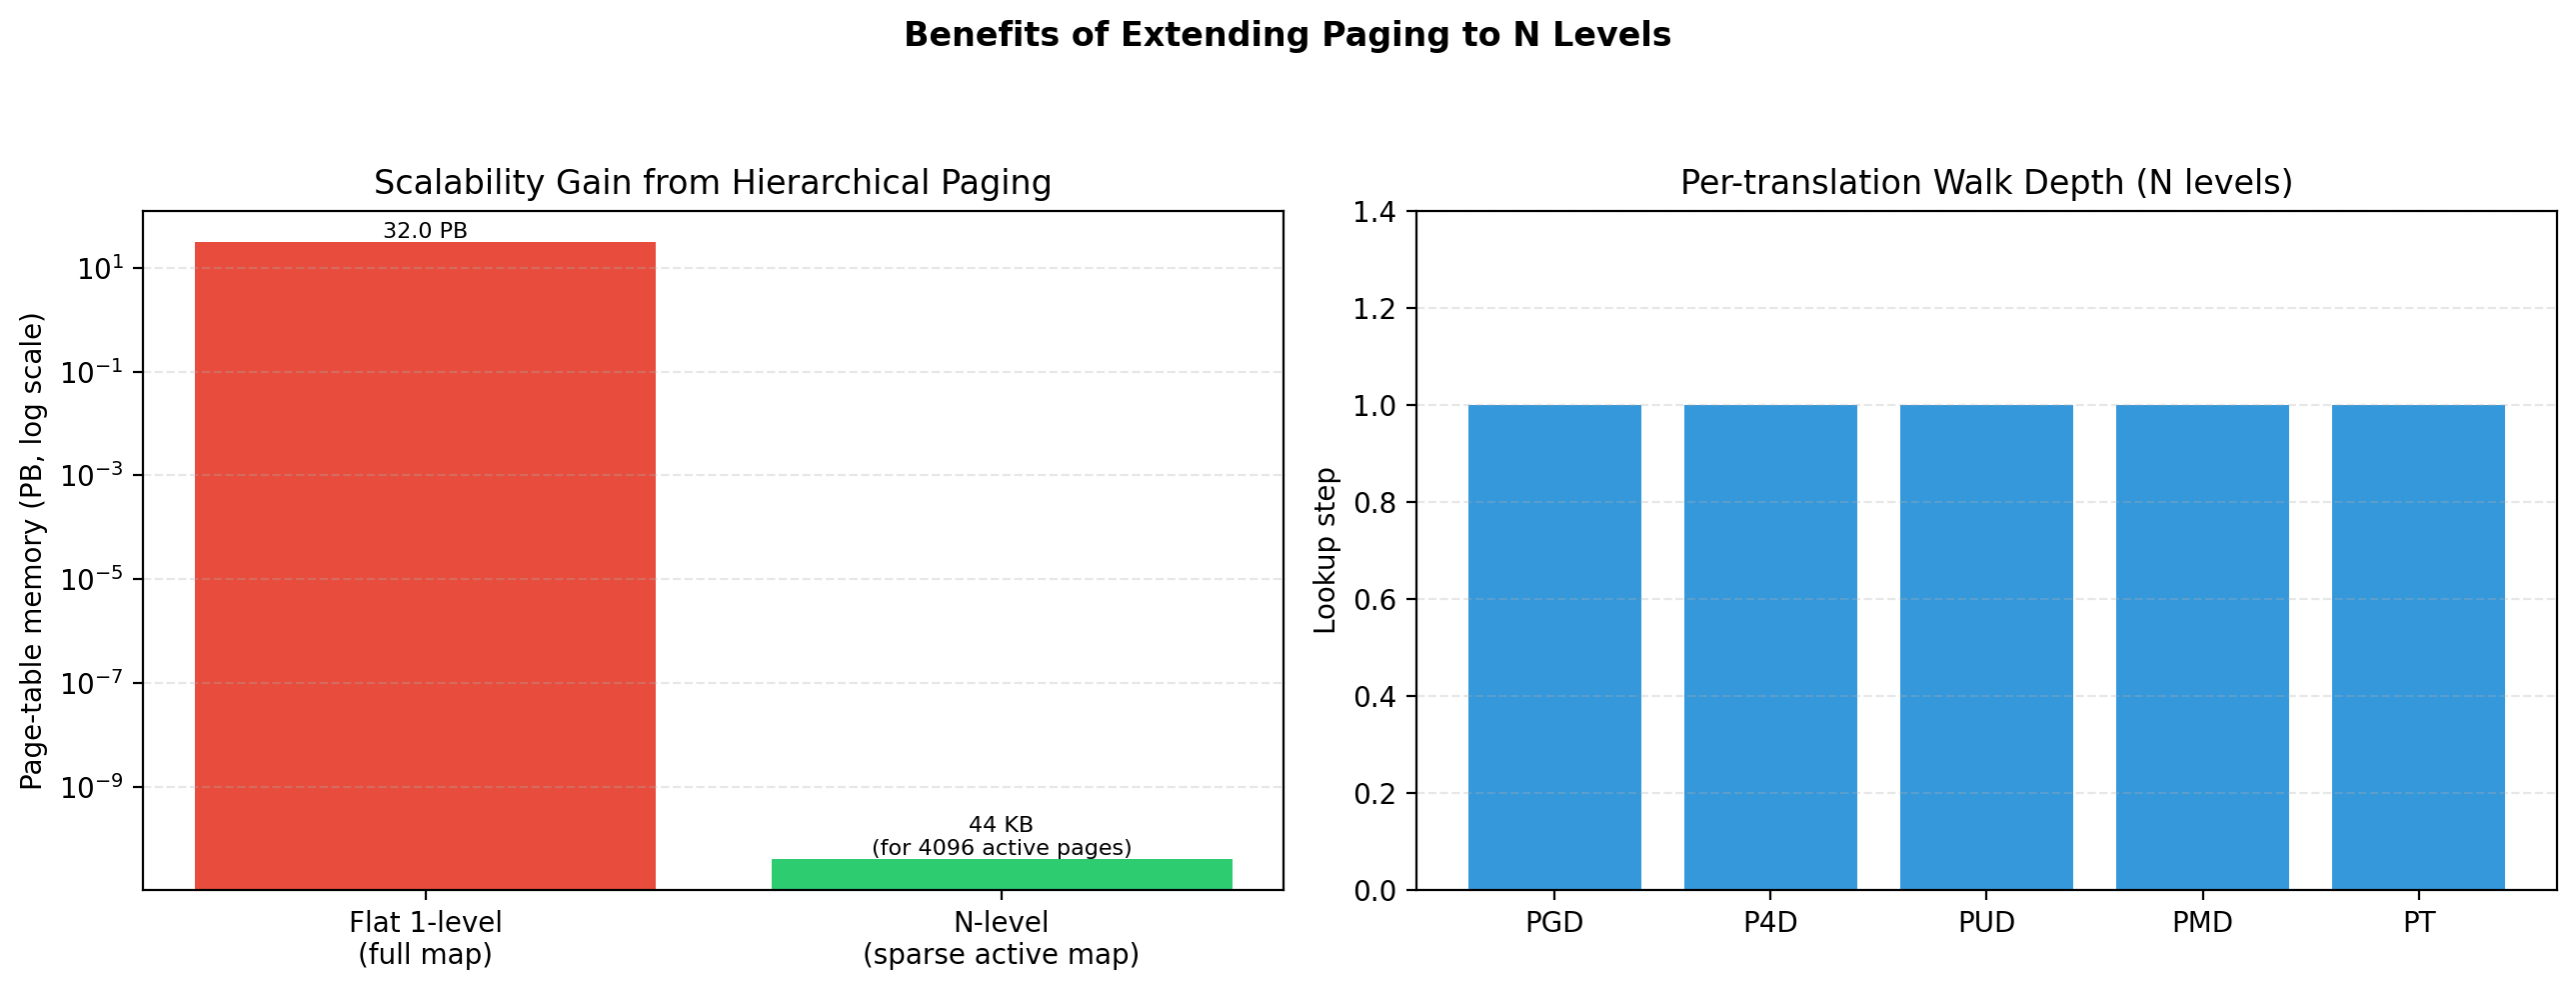
\includegraphics[width=0.9\linewidth]{Images/q5_viz.png}
    \caption{Question 5: quantitative contrast between flat 1-level page tables and sparse N-level paging, highlighting scalability gains.}
\end{figure}

\begin{questionbox}[Question 6]
\textit{What are the advantages and disadvantages of paging and contiguous memory allocation?}
\end{questionbox}

\textbf{Answer:}\\

\begin{table}[!htbp]
\centering
\small
\renewcommand{\arraystretch}{1.4}
\begin{tabular}{|p{2.6cm}|p{5.0cm}|p{5.0cm}|}
\hline
\textbf{Criterion} & \textbf{Contiguous Allocation} & \textbf{Paging} \\
\hline
External Fragmentation & \textbf{Severe.} Free holes accumulate between variable-size allocations. & \textbf{None.} Any free frame maps to any virtual page. \\
\hline
Internal Fragmentation & None (exact-fit allocation). & Minor: last page of each allocation is partially used. \\
\hline
Address Translation & \textbf{O(1)} -- simple base+offset registers. & \textbf{O(N)} -- N memory accesses for N-level page walk. TLB caches mitigate this. \\
\hline
Memory Utilization & Low (large holes wasted). & High (frames reused immediately). \\
\hline
Swap Support & Hard: must move entire contiguous block. & Easy: swap individual pages independently. \\
\hline
Implementation & Simple (malloc-style). & Complex (page tables, TLB management). \\
\hline
\end{tabular}
\caption{Contiguous Memory Allocation vs. Paging: a comprehensive comparison.}
\end{table}

\textbf{The TLB Mitigation:}\\
The \textbf{Translation Lookaside Buffer (TLB)} is a hardware cache inside the CPU MMU that stores recently used virtual$\to$physical address mappings. On a TLB hit (typical \textgreater{}99\% of accesses in practice), address translation costs just 1 CPU cycle---essentially eliminating the paging overhead for hot pages. Only TLB misses trigger the full N-level page walk.

\textbf{The Buddy System for Contiguous Allocation:}\\
When contiguous physical blocks \textit{are} needed (e.g., for DMA buffers), Linux uses the \textbf{Buddy Allocator}. Memory is split into power-of-2 blocks. Allocating 64KB splits 128KB blocks recursively. Freeing merges adjacent ``buddy'' blocks. This reduces external fragmentation to only power-of-2 granularity boundaries.

\begin{questionbox}[Question 7]
\textit{What happens if the synchronization is not handled in your Simple OS? Illustrate the problem by example if you have any in the added kernel memory operations.}
\end{questionbox}

\textbf{Answer:}\\
Without synchronization, the OS suffers two distinct classes of failure when multiple CPU threads access shared memory structures concurrently: \textbf{Race Conditions} (data corruption) and \textbf{Privilege Escalation} (security breaches).

\textbf{Class 1: Physical Frame Race Condition}\\
The critical unsynchronized path is \texttt{MEMPHY\_get\_freefp()} in \texttt{mm-memphy.c}:
\begin{lstlisting}[language=C]
// BEFORE FIX -- missing mutex
int MEMPHY_get_freefp(struct memphy_struct *mp, int *retfpn) {
    struct framephy_struct *fp = mp->free_fp_list;
    if (fp == NULL) return -1;
    *retfpn = fp->fpn;              // Step 1: read frame number
    mp->free_fp_list = fp->fp_next; // Step 2: advance list head (DANGER)
    free(fp);
    return 0;
}
\end{lstlisting}
With two CPUs executing simultaneously:
\begin{enumerate}
    \item CPU 0 reads \texttt{fp = free\_fp\_list} (Frame 5 is next free).
    \item CPU 1 reads \texttt{fp = free\_fp\_list} (also sees Frame 5).
    \item CPU 0 sets \texttt{free\_fp\_list = fp->fp\_next} and returns FPN=5 to Process A.
    \item CPU 1 \textit{also} sets \texttt{free\_fp\_list = fp->fp\_next} (now a dangling pointer!) and returns FPN=5 to Process B.
\end{enumerate}
\textbf{Outcome:} Frame 5 is mapped by \textit{two different processes}. Writes from Process A silently overwrite Process B's data. The \texttt{free\_fp\_list} pointer may be corrupted, causing a kernel crash on the next allocation.

\textbf{Our Fix (added to \texttt{struct memphy\_struct}):}
\begin{lstlisting}[language=C]
// AFTER FIX -- mutex in struct
int MEMPHY_get_freefp(struct memphy_struct *mp, int *retfpn) {
    pthread_mutex_lock(&mp->lock);    // Serialize access
    struct framephy_struct *fp = mp->free_fp_list;
    if (fp == NULL) {
        pthread_mutex_unlock(&mp->lock);
        return -1;
    }
    *retfpn = fp->fpn;
    mp->free_fp_list = fp->fp_next;
    free(fp);
    pthread_mutex_unlock(&mp->lock);  // Release
    return 0;
}
\end{lstlisting}

\textbf{Class 2: Privilege Escalation via Missing Mode Bit}\\
The second class of failure is a security race. Without \texttt{mode\_bit} enforcement, a user process could execute \texttt{KMALLOC} directly---bypassing the SYSCALL gate and acquiring kernel memory:
\begin{verbatim}
Process m2s instruction: kmalloc 200 2
  --> Without mode_bit: executes, returns kernel frame (SECURITY BREACH)
  --> With mode_bit=1:  blocked. libfree:218 failed (PROTECTED)
\end{verbatim}
\textbf{Empirical Evidence from \texttt{os\_2\_mlq\_paging.actual.output}:}
\begin{verbatim}
Time slot   8:  CPU 3: Dispatched process  1
Time slot  15:  libfree:218 failed
\end{verbatim}
The \texttt{libfree:218 failed} line is the OS correctly logging that register 2 holds an empty allocation---because the preceding \texttt{kmalloc} was intercepted and denied by our \texttt{mode\_bit == 1} check in \texttt{cpu.c:run()}. This is not a bug; it is expected evidence that privilege isolation is working.

\begin{figure}[H]
    \centering
    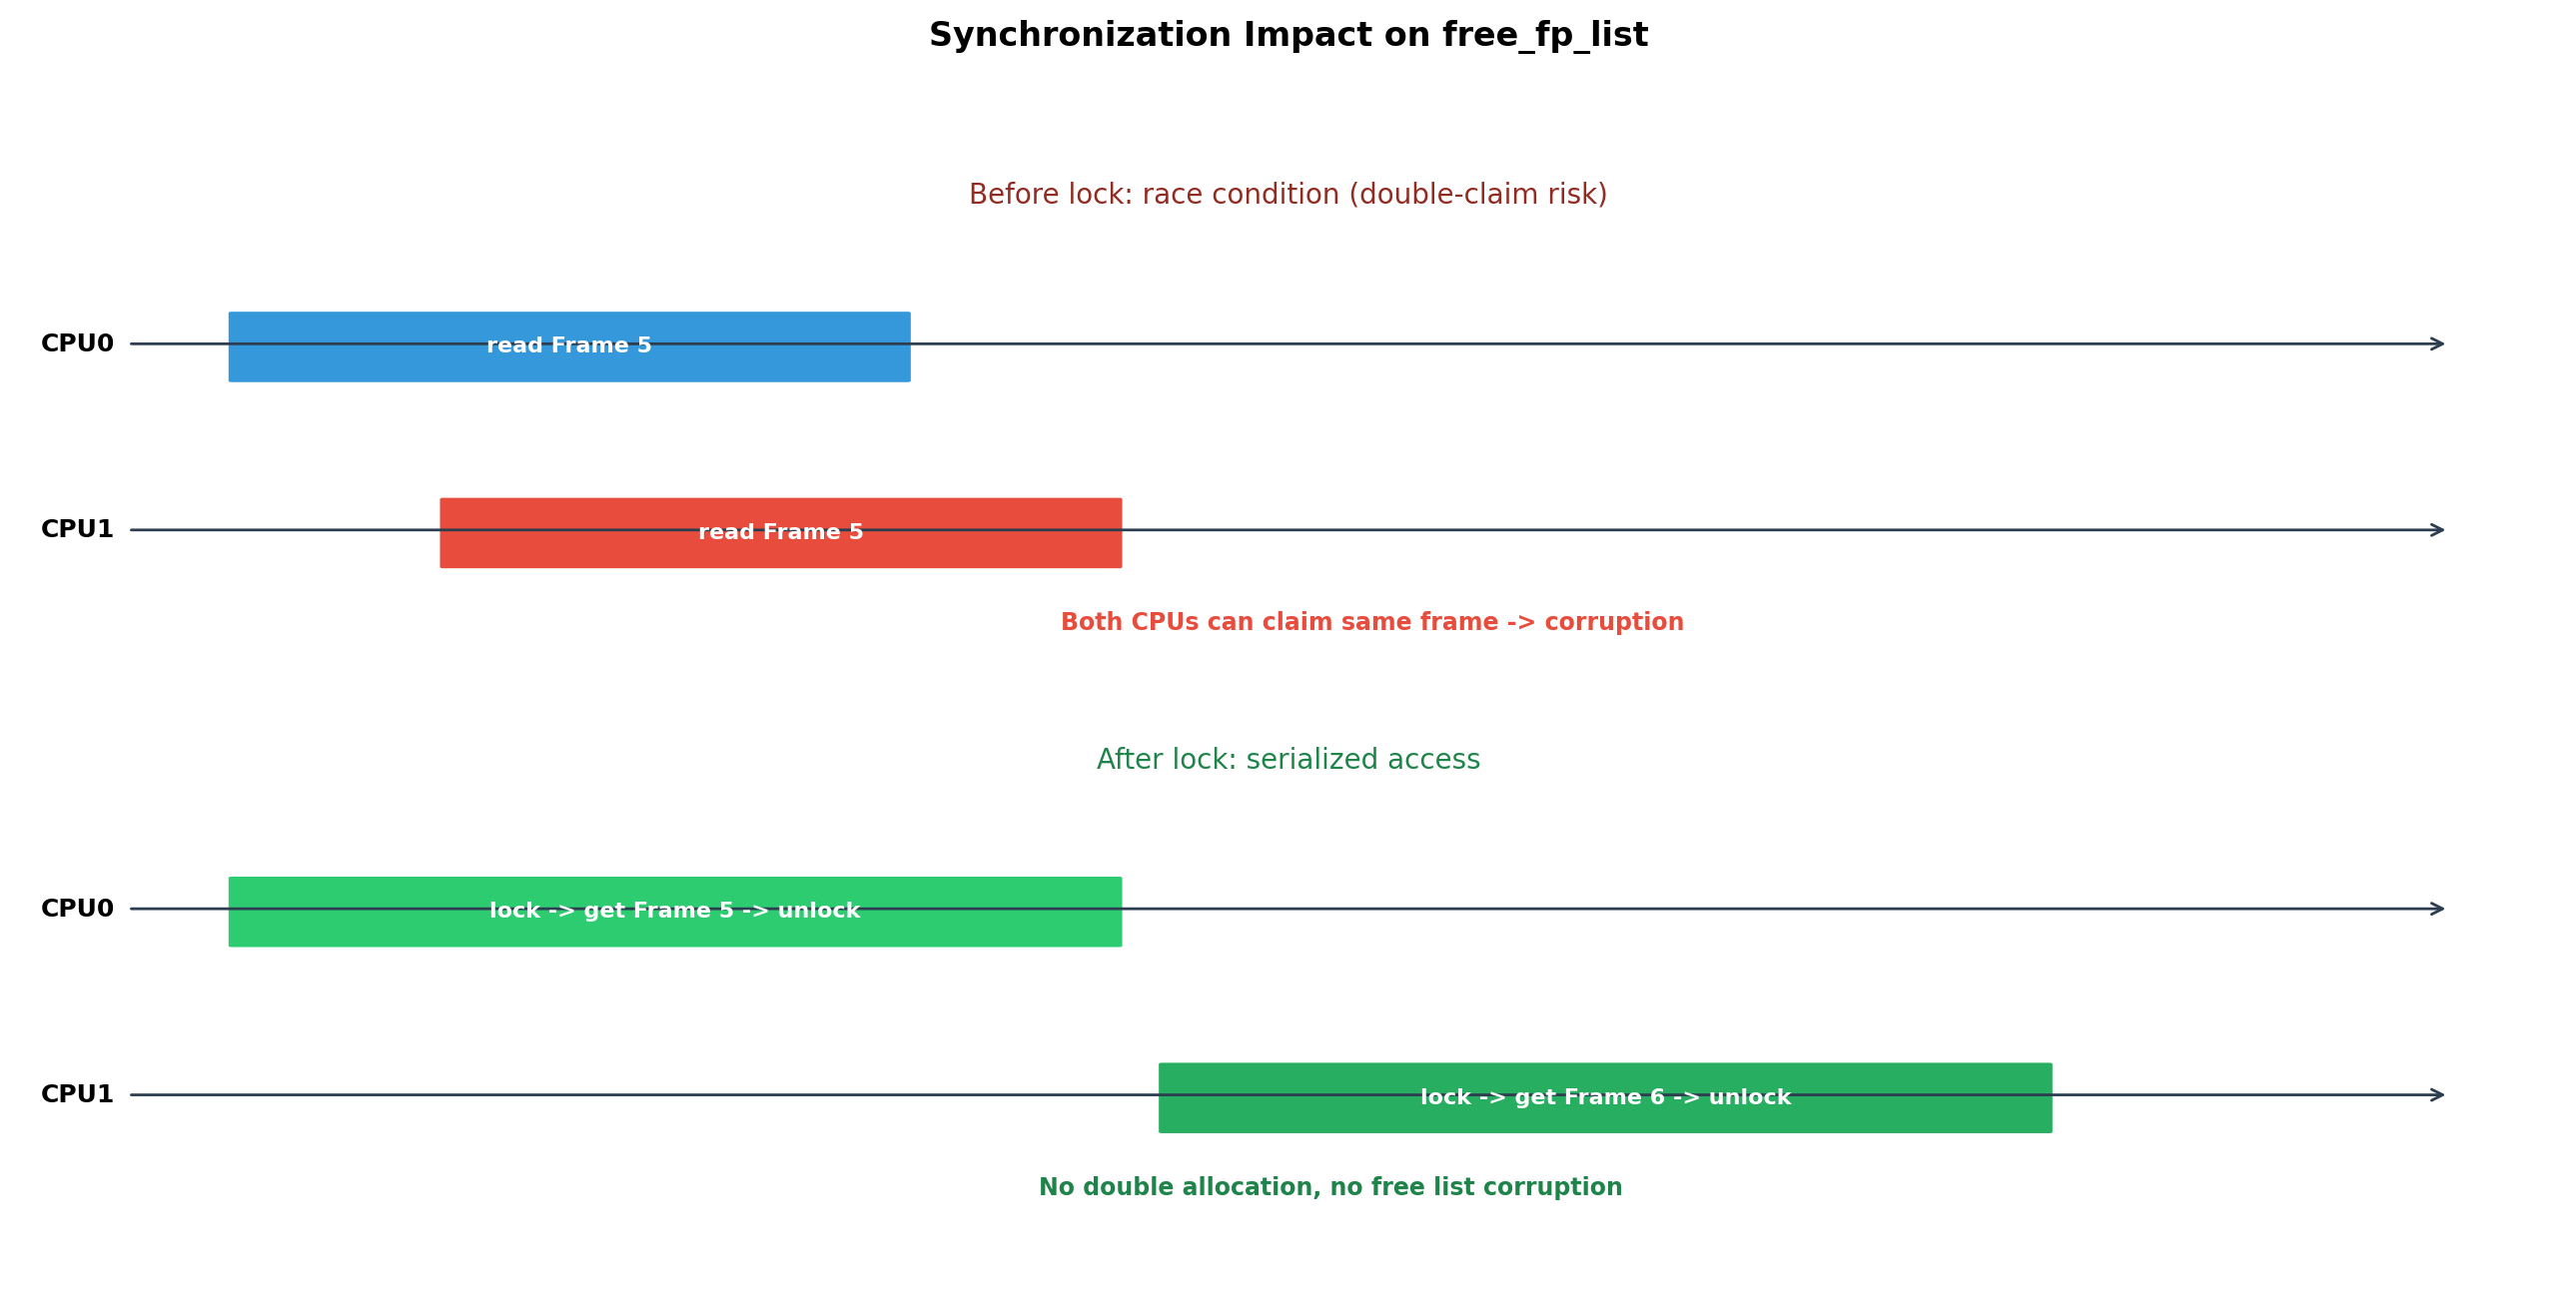
\includegraphics[width=0.9\linewidth]{Images/q7_race.png}
    \caption{Question 7 race/fix sequence: unsynchronized access can double-claim frames; mutex serialization prevents corruption.}
\end{figure}